\begin{frame}{Vectors}
\begin{itemize}
    \item Recap: Vectors are a sequence of numbers
    $$[1.0, 2.0]; [6.0, 5.3, 2.1, -6.7]$$
    \item Vector Spaces
    $$\mathbb{R}^2 = \{(x, y) : x, y \in \mathbb{R}\}$$
    $$\mathbb{R}^4 = \{(a, b, c, d) : a, b, c, d \in \mathbb{R}\}$$
    \begin{figure}
    \centering
    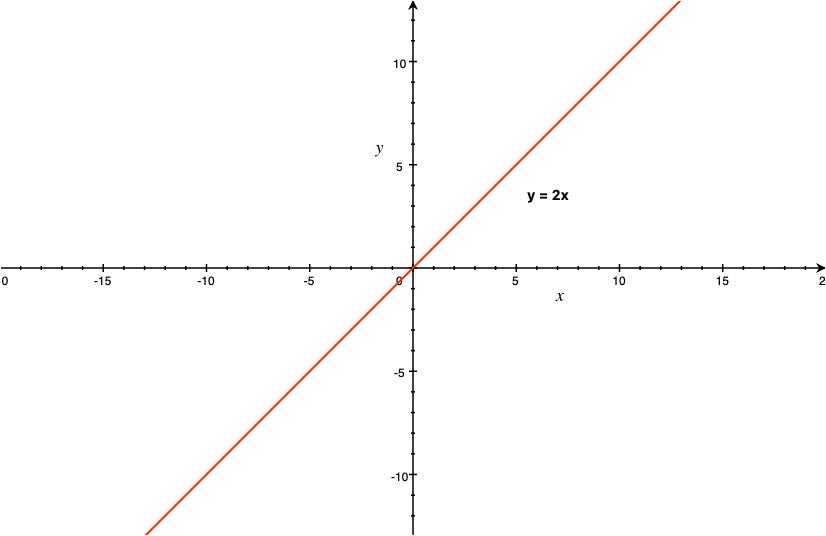
\includegraphics[width=.5\textwidth]{img/line.jpg}
    \caption{Vectors in the 2D plane $(x, y)$ are in $\mathbb{R}^2$}
    \end{figure}
\end{itemize}
\end{frame}

\begin{frame}{Linear Models for Regression}
\begin{figure}
    \centering
    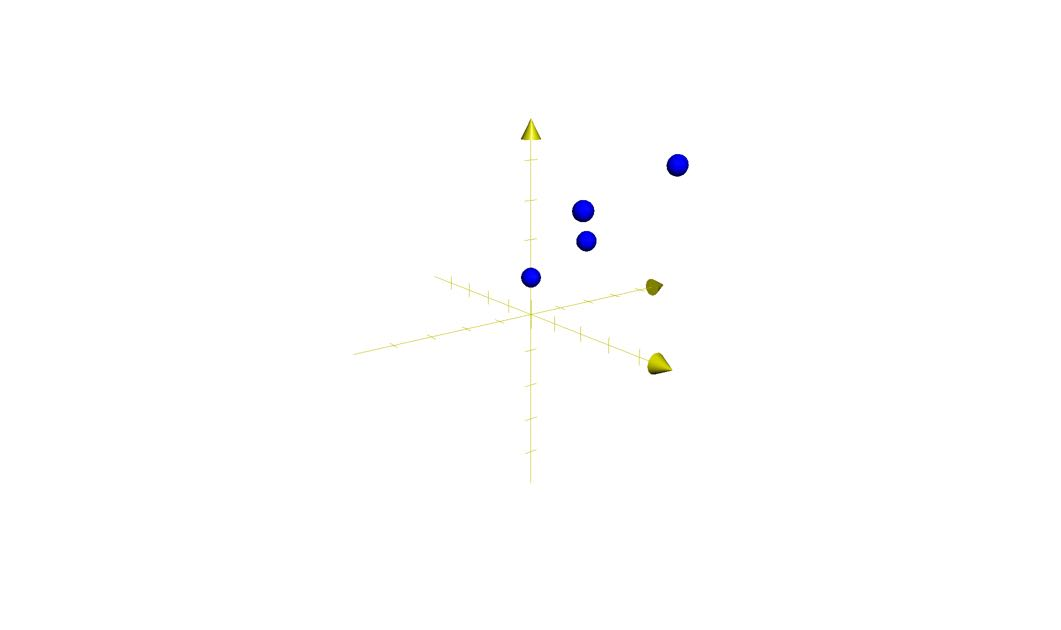
\includegraphics[width=0.9\textwidth]{img/3d_regressed_points.jpg}
    \caption{3D blue point dataset $(x_1, x_2, y) \in \mathbb{R}^3$}
\end{figure}
\end{frame}

\begin{frame}{Vectors}
\begin{itemize}
    \item In logistic regression: $\hat{y} = \sigma(w_0 + w_1x_1 + ... + w_Dx_D)$
    $$\textbf{w} = (w_0, ..., w_D) \in \mathbb{R}^D, \textbf{x} = (x_0, ..., x_D) \in \mathbb{R}^D$$
    $$\hat{y} = \sigma(\textbf{w} \cdot \textbf{x})$$
\end{itemize}
\end{frame}

